% Bản dịch tiếng Việt bài báo HFR-MKGC (AAAI 2026).
% Biên dịch: xelatex HFR-MKGC-tieng-viet.tex  (chạy 2 lần để cập nhật tham chiếu)
\documentclass[10pt,twocolumn,a4paper]{article}

\usepackage{fontspec}
\setmainfont{Times New Roman}
\usepackage{polyglossia}
\setdefaultlanguage{vietnamese}
\usepackage[margin=2cm,top=2.2cm,bottom=2.2cm]{geometry}
\usepackage{amsmath,amssymb}
\usepackage{graphicx}
\usepackage{booktabs}
\usepackage{multirow}
\usepackage{caption}
\usepackage{enumitem}
\usepackage[hidelinks]{hyperref}
\usepackage{xcolor}
\usepackage{microtype}

\graphicspath{{figures/}}
\captionsetup{font=small,labelfont=bf}
\setlength{\columnsep}{0.6cm}
\setlist{nosep,leftmargin=*}

\newcommand{\Prom}{\mathrm{Prom}}
\newcommand{\Hj}{\mathbf{H}_{\mathrm{joint}}}
\newcommand{\Tj}{\mathbf{T}_{\mathrm{joint}}}
\newcommand{\Tm}{\mathbf{T}_{\mathrm{MLLM}}}
\renewcommand{\Re}{\operatorname{Re}}
\renewcommand{\Im}{\operatorname{Im}}
\newcommand{\score}{\mathrm{score}}

\title{\textbf{HFR-MKGC: Suy luận hợp nhất phân cấp với MLLM cho bài toán hoàn thiện đồ thị tri thức đa phương thức}\\[4pt]
\large\textit{HFR-MKGC: Hierarchical Fusion Reasoning with MLLMs for Multi-modal Knowledge Graph Completion}}

\author{Di Wang$^{1,2}$, Junping Du$^{1,2*}$, Zhe Xue$^{1,2}$, Meiyu Liang$^{1,2}$, Guanhua Ye$^{1,2}$, Yingxia Shao$^{1,2}$, Haisheng Li$^{3}$\\[3pt]
\small $^1$School of Computer Science (National Pilot School of Software Engineering), Beijing University of Posts and Telecommunications\\
\small $^2$Beijing Key Laboratory of Intelligent Telecommunication Software and Multimedia\\
\small $^3$School of Computer and Artificial Intelligence, Beijing Technology and Business University\\[3pt]
\small \{wdd123, xuezhe, meiyu1210, g.ye, shaoyx\}@bupt.edu.cn, junpingdu@126.com, lihsh@btbu.edu.cn\\[4pt]
\small\textit{Bản dịch tiếng Việt phục vụ seminar. Nguồn: The Fortieth AAAI Conference on Artificial Intelligence (AAAI-26), tr.~15815--15823.}}
\date{}

\begin{document}
\maketitle

\begin{abstract}
\noindent
Hoàn thiện đồ thị tri thức đa phương thức (Multi-modal Knowledge Graph Completion, MMKGC) nhằm suy ra thực thể còn thiếu của bộ ba bằng cách khai thác thông tin không đồng nhất trong đồ thị tri thức (Knowledge Graph, KG). Tuy nhiên, các phương pháp hiện có thường gặp khó khăn với việc căn chỉnh phương thức thiếu nhất quán, độ sâu suy luận hạn chế và chất lượng mẫu âm không đủ tốt. Trong công trình này, chúng tôi đề xuất HFR-MKGC, một khung mới tích hợp hợp nhất phương thức phân cấp và suy luận bằng mô hình ngôn ngữ lớn đa phương thức (Multimodal Large Language Model, MLLM) để MMKGC bền vững và giàu biểu đạt. Cụ thể, chúng tôi đưa ra mô-đun hợp nhất phương thức phân cấp có dẫn hướng bởi quan hệ, thực hiện hợp nhất tinh trong nội bộ phương thức thị giác và tích hợp liên phương thức theo quan hệ để tạo biểu diễn thực thể giàu thông tin. HFR-MKGC dùng một MLLM đã tinh chỉnh để suy luận bộ ba theo chỉ dẫn, sinh ra các thực thể ứng viên cho việc hoàn thiện. Sau đó, nó xây dựng các mẫu âm khó thông qua nhiễu loạn văn bản bằng MLLM và tăng cường đặc trưng thị giác bằng phép xoay và nhiễu. HFR-MKGC tối ưu mô hình bằng huấn luyện đối kháng. Thực nghiệm rộng rãi trên ba bộ dữ liệu chuẩn MMKGC cho thấy phương pháp của chúng tôi vượt các phương pháp tiên tiến nhất, xác nhận hiệu quả của nó trong MMKGC.
\end{abstract}

\section{Giới thiệu}

Đồ thị tri thức (KG) lưu trữ các sự thật trong thế giới thực dưới dạng bộ ba $(h, r, t)$, trong đó $h$, $t$ và $r$ lần lượt là thực thể đầu, thực thể đuôi và quan hệ giữa chúng. Dù được sử dụng rộng rãi trong hỏi đáp (Panda et al. 2024; Wang et al. 2025), hệ gợi ý (Cui et al. 2025; Xiao et al. 2022) và tìm kiếm ngữ nghĩa (Liang et al. 2024a,b), KG thường thiếu hoàn chỉnh. Các phương pháp hoàn thiện đồ thị tri thức (Knowledge Graph Completion, KGC) truyền thống (Bordes et al. 2013; Sun et al. 2019; Yang et al. 2015; Trouillon et al. 2016) chủ yếu dựa vào thông tin cấu trúc, bỏ qua các gợi ý ngữ nghĩa bổ sung từ những phương thức khác.

Để giải quyết điều này, MMKGC tận dụng thêm các phương thức như văn bản và hình ảnh để dự đoán bộ ba chưa hoàn chỉnh. Các phương pháp MMKGC điển hình nhúng thực thể và quan hệ từ nhiều phương thức vào một không gian vector chung (Gao et al. 2025) và dùng một hàm điểm để xếp hạng các bộ ba ứng viên. Các hướng tiếp cận tiêu biểu gồm chiến lược hợp nhất sớm, nối hoặc lấy trung bình trực tiếp các embedding phương thức (Mousselly-Sergieh et al. 2018), và các phương pháp hợp nhất nâng cao, học biểu diễn chung qua cơ chế chú ý (Chen et al. 2022), mô-đun cổng (Wang et al. 2021) hoặc tích hợp đa cấp (Wang et al. 2019). Hơn nữa, một số phương pháp xây dựng mẫu âm khó đa phương thức cho huấn luyện đối kháng bằng cách tiêm nhiễu hoặc nhiễu loạn (Zhang, Chen, and Zhang 2023; Zhang et al. 2024c; Chen et al. 2025a). Gần đây, sự tiến bộ nhanh chóng của mô hình ngôn ngữ lớn (Large Language Model, LLM) đã gợi mở những hướng tiếp cận mới cho KGC. Bằng cách chuyển thông tin cấu trúc và văn bản của KG thành prompt ngôn ngữ tự nhiên (Fang et al. 2024; Barile, d'Amato, and Fanizzi 2025; Pan et al. 2025; Zhang et al. 2024b; Yao et al. 2025), LLM có thể suy luận để suy ra các bộ ba còn thiếu hợp lý.

\begin{figure}[t]
\centering
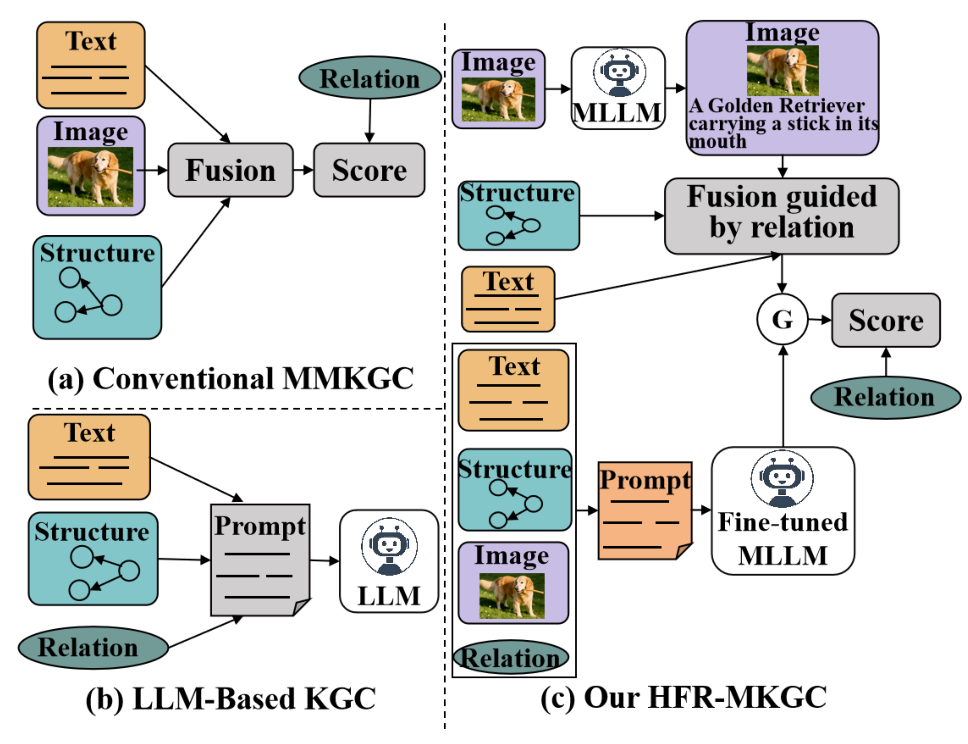
\includegraphics[width=\linewidth]{fig1}
\caption{So sánh ba mô hình (paradigm) MMKGC.}
\label{fig:paradigms}
\end{figure}

Dù nghiên cứu MMKGC đã tiến bộ, các phương pháp hiện có vẫn đối mặt với hai thách thức chính: \textbf{(1) Thiếu hợp nhất đa phương thức có dẫn hướng bởi quan hệ.} Hầu hết chiến lược hợp nhất đối xử mọi phương thức như nhau, bỏ qua việc tầm quan trọng của mỗi phương thức có thể thay đổi theo từng quan hệ. Thiết kế bất khả tri quan hệ này khiến mô hình dễ bị ảnh hưởng bởi phương thức nhiễu hoặc không liên quan, đặc biệt khi thông tin thị giác hoặc văn bản liên quan yếu tới quan hệ. \textbf{(2) Khả năng thích ứng hạn chế của suy luận dựa trên LLM.} Các phương pháp KGC có LLM hỗ trợ hiện nay chủ yếu tập trung vào phương thức văn bản và cấu trúc, thường dựa vào chiến lược hợp nhất tĩnh. Thiết kế như vậy không khai thác đầy đủ ngữ nghĩa thị giác và không thể thích ứng động với mức độ liên quan thay đổi của các phương thức giữa các bộ ba khác nhau.

Để giải quyết các thách thức nêu trên, chúng tôi đề xuất phương pháp có tên Hierarchical Fusion Reasoning with MLLMs for Multi-modal Knowledge Graph Completion (HFR-MKGC). Để minh hoạ rõ khoảng cách giữa các phương pháp thông thường và phương pháp đề xuất, chúng tôi so sánh ba mô hình trong Hình~\ref{fig:paradigms}: khung MMKGC thông thường, khung KGC dựa trên LLM và khung HFR-MKGC của chúng tôi. HFR-MKGC sử dụng một MLLM để suy luận phụ trợ và đề xuất hai chiến lược sau: \textbf{(1) Hợp nhất phương thức phân cấp có dẫn hướng bởi quan hệ (Relation-Guided Hierarchical Modal Fusion).} Chúng tôi dùng một MLLM để sinh mô tả văn bản chi tiết cho ảnh của mỗi thực thể và hợp nhất chúng với embedding thị giác, nắm bắt các gợi ý thị giác--ngữ nghĩa bổ trợ. Sau đó, một cơ chế hợp nhất liên phương thức có dẫn hướng bởi quan hệ sẽ gán trọng số thích ứng cho các phương thức văn bản, thị giác và cấu trúc dựa trên quan hệ hiện tại, cho phép hợp nhất bền vững đồng thời triệt tiêu tín hiệu không liên quan hoặc nhiễu. \textbf{(2) Suy luận và chấm điểm tri thức tăng cường bằng MLLM (MLLMs-Enhanced Knowledge Reasoning and Scoring).} Chúng tôi tận dụng một MLLM đã tinh chỉnh để suy luận riêng cho từng bộ ba, sinh ra các thực thể đuôi ứng viên dựa trên gợi ý cấu trúc, văn bản và thị giác. Các kết quả suy luận này được tích hợp vào hàm điểm cuối cùng qua một cơ chế cổng, cho phép mô hình thích ứng chiến lược suy luận với các kịch bản suy diễn đa dạng. Cuối cùng, chúng tôi xây dựng mẫu âm khó qua nhiễu loạn và tăng cường đa phương thức, rồi tối ưu toàn bộ mô hình trong khung huấn luyện đối kháng để tăng thêm tính bền vững và khả năng khái quát hoá. Các đóng góp chính của công trình được tóm tắt như sau:
\begin{itemize}
\item Chúng tôi đề xuất HFR-MKGC, một khung mới cho MMKGC, cho phép hợp nhất tinh trong nội bộ phương thức thị giác và gán trọng số đặc trưng liên phương thức có dẫn hướng bởi quan hệ, triệt tiêu hiệu quả các phương thức không liên quan hoặc nhiễu. HFR-MKGC còn tăng tính bền vững thông qua huấn luyện đối kháng với mẫu âm đa phương thức.
\item Chúng tôi thiết kế chiến lược Suy luận và chấm điểm tri thức tăng cường bằng MLLM mới, trong đó một MLLM đã tinh chỉnh suy luận riêng cho từng bộ ba và kết quả suy luận được tích hợp vào quá trình chấm điểm, cho phép suy luận thích ứng trong nhiều kịch bản suy diễn.
\item Chúng tôi thực hiện thực nghiệm toàn diện và phân tích sâu trên ba bộ dữ liệu MMKGC công khai, cho thấy HFR-MKGC đạt hiệu năng SOTA so với 14 mô hình cơ sở.
\end{itemize}

\section{Nghiên cứu liên quan}

Để cung cấp bối cảnh đầy đủ, chúng tôi giới thiệu ngắn gọn về MMKGC và việc sử dụng đang nổi lên của LLM, đặc biệt là MLLM, cho các tác vụ suy luận tri thức trên KG.

\subsection{Hoàn thiện đồ thị tri thức đa phương thức}

Các phương pháp MMKGC tích hợp các phương thức bổ trợ như văn bản (Xie et al. 2016) và hình ảnh (Xie et al. 2017) để làm giàu biểu diễn thực thể và quan hệ. Các chiến lược phổ biến gồm nối vector đơn giản (Mousselly-Sergieh et al. 2018), mô hình hoá đồ thị không đồng nhất (Zhao et al. 2025; Wang et al. 2025) và học embedding chung (Li, Yu, and He 2024; Li et al. 2023). TransAE (Wang et al. 2019) mã hoá đồng thời đặc trưng văn bản và thị giác qua một bộ tự mã hoá đa phương thức. MKGformer (Chen et al. 2022) đưa ra hợp nhất phân cấp để lọc nhiễu thị giác không liên quan, trong khi RSME (Wang et al. 2021) dùng cơ chế cổng để triệt tiêu các phương thức không mang thông tin. MCKGC (Gao et al. 2025) nhúng các phương thức vào nhiều không gian hình học khác nhau và dùng cổng phân cấp để tích hợp. MACO (Zhang, Chen, and Zhang 2023) xử lý kịch bản thiếu phương thức bằng cách thêm nhiễu vào góc nhìn thị giác và cấu trúc để mô phỏng mẫu âm. AdaMF-MAT (Zhang et al. 2024c) học trọng số hợp nhất thích ứng giữa các phương thức qua tối ưu đối kháng, và NativeE (Zhang et al. 2024a) mở rộng ý tưởng này sang các phương thức số, âm thanh và video trong một khung huấn luyện thống nhất. Các mô hình dựa trên nhiễu (Chen et al. 2025a; Jian et al. 2025) và dựa trên khuếch tán (Chen et al. 2025b) để sinh mẫu âm còn cải thiện thêm khả năng khái quát hoá.

Hầu hết công trình trước đây dùng hợp nhất bất khả tri quan hệ và dễ bị nhiễu. Ngược lại, chúng tôi đưa ra cơ chế hợp nhất phân cấp có dẫn hướng bởi quan hệ, cho phép căn chỉnh tinh và nhấn mạnh thích ứng các gợi ý ngữ nghĩa liên quan nhất tới quan hệ.

\subsection{Mô hình ngôn ngữ lớn cho suy luận tri thức}

Những năm gần đây, LLM đã cho thấy tiềm năng đáng kể trong suy luận tri thức để tích hợp các nguồn thông tin đa dạng (Zhang et al. 2024d). GAugLLM (Fang et al. 2024) cải thiện học tự giám sát trên đồ thị có thuộc tính văn bản bằng tăng cường dựa trên prompt. Một số nghiên cứu chuyển cấu trúc KG thành dạng văn bản mà LLM hiểu được để căn chỉnh thực thể (Jiang et al. 2024; Zhang et al. 2023) và KGC (Zhang et al. 2024b; Yao et al. 2025). LP-DIXIT (Barile, d'Amato, and Fanizzi 2025) đánh giá khả năng giải thích của kết quả dự đoán liên kết bằng LLM. Hơn nữa, LoLLM (Pan et al. 2025) tích hợp LLM với embedding cấu trúc để suy luận trên KG thưa. HOLMES (Panda et al. 2024) tích hợp một KG đã chưng cất và nhận biết ngữ cảnh vào LLM để hỗ trợ hỏi đáp. Gần đây, các nhà nghiên cứu đã kết hợp MMKG với LLM. UniMEL (Liu et al. 2024) đề xuất khung đa phương thức thống nhất dựa trên LLM, hợp nhất hiệu quả thông tin văn bản và thị giác cho liên kết thực thể. Ngoài ra, MuKDC (Li et al. 2024) tăng cường KGC ít mẫu (few-shot) qua sinh tri thức đa cấp, còn CATS (Li et al. 2025) cải thiện KGC quy nạp (inductive) bằng LLM.

Suy luận KG dựa trên LLM hiện có chủ yếu tập trung vào phương thức văn bản và cấu trúc với hợp nhất tĩnh, hạn chế khả năng thích ứng. Chúng tôi mở rộng sang MLLM để suy luận tri thức thống nhất trên các phương thức cấu trúc, văn bản và thị giác, với cơ chế cổng để hợp nhất động theo từng bộ ba nhằm nâng cao hiệu năng MMKGC.

\begin{figure*}[t]
\centering
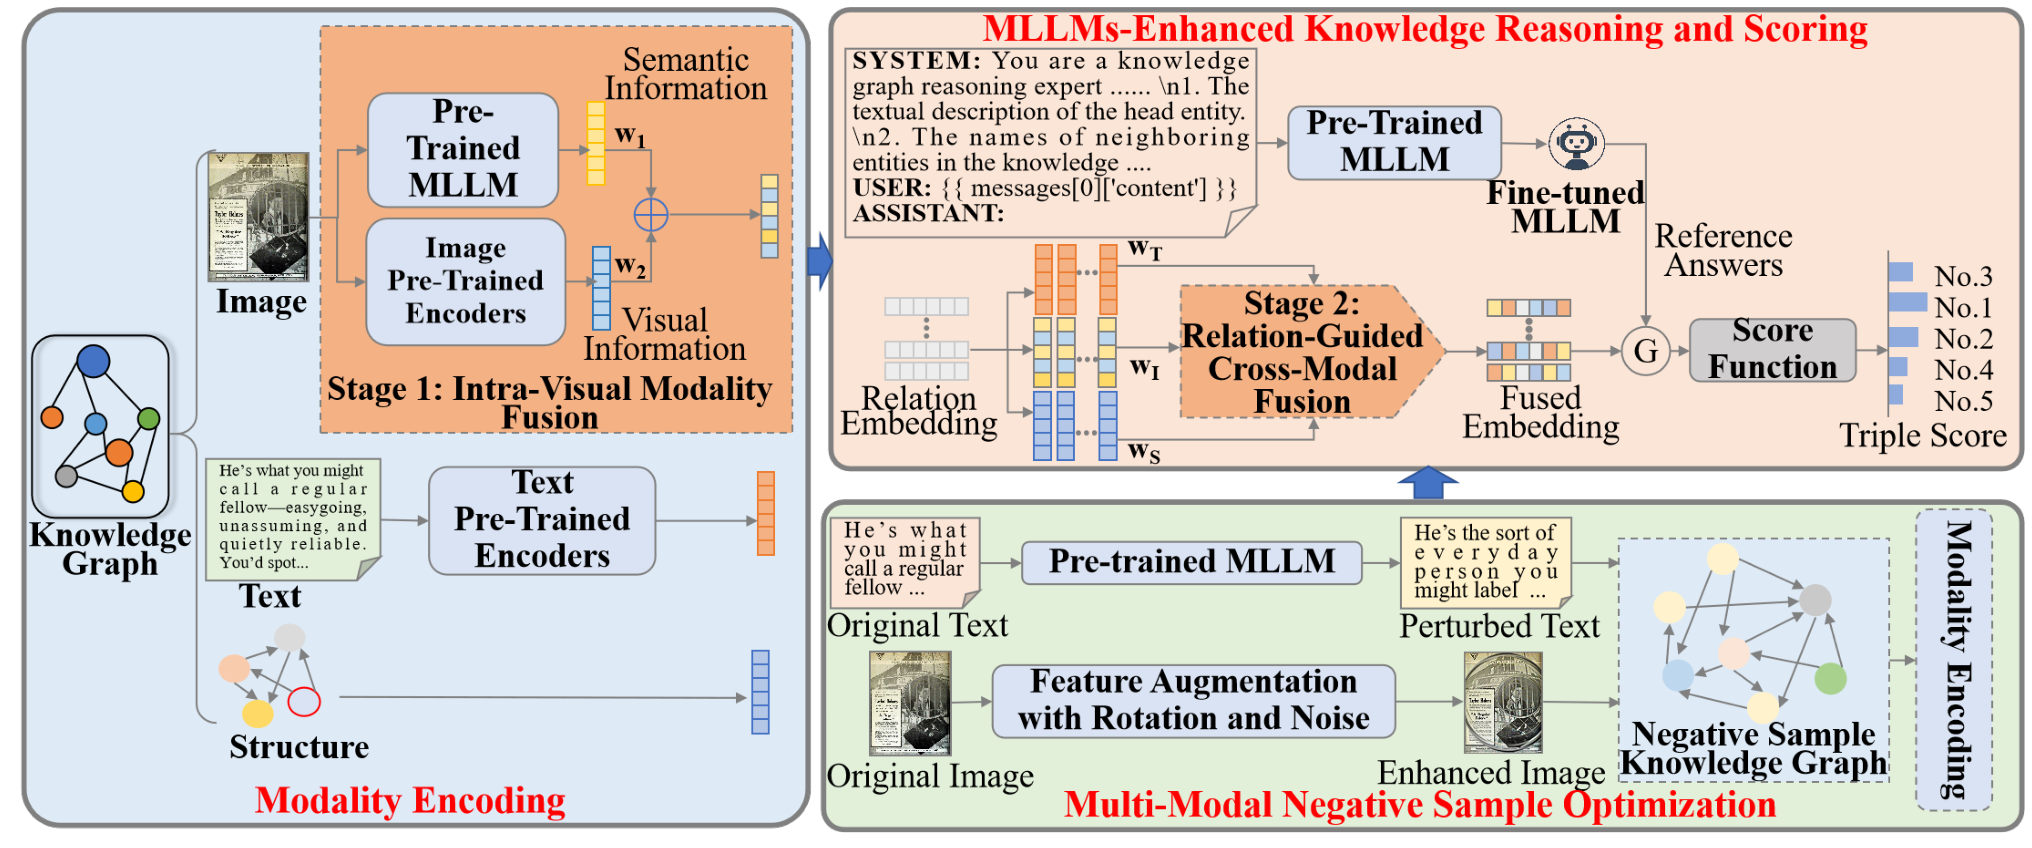
\includegraphics[width=\textwidth]{fig2}
\caption{Khung tổng thể của HFR-MKGC. (1) Giai đoạn 1: Hợp nhất nội bộ phương thức thị giác (Intra-Visual Modality Fusion) và Giai đoạn 2: Hợp nhất liên phương thức có dẫn hướng bởi quan hệ (Relation-Guided Cross-Modal Fusion) tạo thành mô-đun Hợp nhất phương thức phân cấp có dẫn hướng bởi quan hệ, thực hiện hợp nhất tinh trong nội bộ phương thức rồi gán trọng số theo quan hệ để tích hợp liên phương thức. (2) Suy luận và chấm điểm tri thức tăng cường bằng MLLM: một MLLM đã tinh chỉnh sinh thực thể ứng viên cho bộ ba chưa hoàn chỉnh, kết quả suy luận được hợp nhất với embedding đa phương thức để chấm điểm cuối cùng. (3) Tối ưu mẫu âm đa phương thức: mẫu âm khó được xây dựng qua nhiễu loạn văn bản bằng MLLM và tăng cường đặc trưng thị giác bằng phép xoay và nhiễu, mô hình được huấn luyện bằng học đối kháng để tăng tính bền vững và khả năng phân biệt.}
\label{fig:framework}
\end{figure*}

\section{Định nghĩa bài toán}

Một MMKG được định nghĩa là $\mathcal{G} = (\mathcal{E}, \mathcal{R}, \mathcal{T})$, trong đó $\mathcal{E}$ là tập thực thể, $\mathcal{R}$ là tập quan hệ, và $\mathcal{T} = \{(h, r, t) \mid h, t \in \mathcal{E},\ r \in \mathcal{R}\}$ là tập bộ ba. Mỗi thực thể $e \in \mathcal{E}$ có thể gắn với thông tin đa phương thức $\mathcal{M}_e = \{T, I, S\}$, lần lượt biểu thị mô tả văn bản, hình ảnh và ngữ cảnh cấu trúc. Một bộ ba chưa hoàn chỉnh cũng được gọi là bộ ba truy vấn (query triple). Bài toán MMKGC nhằm dự đoán thực thể còn thiếu trong bộ ba truy vấn (ví dụ $(h, r, ?)$ hoặc $(?, r, t)$) bằng cách khai thác các nguồn thông tin đa phương thức này. Điều này đạt được bằng cách học một hàm điểm $f(h, r, t)$ để xếp hạng các thực thể ứng viên và chọn thực thể hợp lý nhất để hoàn thiện.

\section{Phương pháp}

Trong phần này, chúng tôi trình bày chi tiết HFR-MKGC. Như Hình~\ref{fig:framework}, HFR-MKGC gồm ba mô-đun chính: (1) Hợp nhất phương thức phân cấp có dẫn hướng bởi quan hệ; (2) Suy luận và chấm điểm tăng cường bằng MLLM; (3) Tối ưu mẫu âm đa phương thức.

\subsection{Hợp nhất phương thức phân cấp có dẫn hướng bởi quan hệ}

Mô-đun này nhằm tích hợp sâu các đặc trưng đa phương thức thông qua chiến lược hợp nhất hai giai đoạn. Giai đoạn thứ nhất là mức hợp nhất nội bộ phương thức, dùng MLLM để dẫn hướng hợp nhất tinh giữa biểu diễn thị giác và biểu diễn ngữ nghĩa của ảnh. Giai đoạn thứ hai là mức hợp nhất liên phương thức, phân bổ động trọng số hợp nhất liên phương thức dựa trên thông tin quan hệ và sinh ra biểu diễn đặc trưng chung bền vững.

\paragraph{Mã hoá phương thức (Modality Encoding).}
Cho một thực thể $e$ với các phương thức khác nhau, chúng tôi mã hoá đặc trưng thị giác của ảnh bằng CLIP (Radford et al. 2021) và mã hoá đặc trưng văn bản bằng BERT (Devlin et al. 2019). Hơn nữa, với mỗi thực thể $e \in \mathcal{E}$ và phương thức $m \in \mathcal{M}_e$, chúng tôi ký hiệu embedding riêng theo phương thức là $\mathbf{e}_m = P_m(\mathbf{f}_m) \in \mathbb{R}^{d_e}$, trong đó $\mathbf{f}_m$ là đặc trưng ban đầu do bộ mã hoá tiền huấn luyện trích xuất, và $P_m$ là một lớp chiếu (projection layer) có thể học cho phương thức $m$. Một điểm đáng chú ý là chú thích ảnh (caption) được sinh ra cũng được xem là một loại phương thức văn bản.

\paragraph{Giai đoạn 1: Hợp nhất nội bộ phương thức thị giác.}
Để giảm sự thiếu nhất quán bên trong phương thức, chúng tôi dùng một MLLM, LLaVA (Liu et al. 2023), để sinh chú thích mô tả làm thông tin ngữ nghĩa cho ảnh. Chúng tôi mã hoá các chú thích này bằng BERT và chiếu chúng vào không gian đặc trưng thống nhất bằng $P_T$, ký hiệu $\mathbf{e}_{I_c} \in \mathbb{R}^d$. Tương tự, biểu diễn thị giác của ảnh gốc ký hiệu $\mathbf{e}_{I_v} \in \mathbb{R}^d$. Sau đó, chúng tôi dùng cơ chế cổng dựa trên độ tương đồng để thực hiện hợp nhất tinh giữa $\mathbf{e}_{I_c}$ và $\mathbf{e}_{I_v}$, tính như sau:
\begin{equation}
\mathbf{e}_I = \sigma\big(\langle \mathbf{e}_{I_v}, \mathbf{e}_{I_c}\rangle\big)\cdot \mathbf{e}_{I_c} + \Big(1 - \sigma\big(\langle \mathbf{e}_{I_v}, \mathbf{e}_{I_c}\rangle\big)\Big)\cdot \mathbf{e}_{I_v}
\label{eq:1}
\end{equation}
trong đó $\sigma(\cdot)$ là hàm kích hoạt Sigmoid, và $\langle\cdot,\cdot\rangle$ là độ tương đồng tích vô hướng giữa $\mathbf{e}_{I_v}$ và $\mathbf{e}_{I_c}$. Vector hợp nhất thu được $\mathbf{e}_I \in \mathbb{R}^d$ tích hợp cả gợi ý thị giác mức thấp lẫn ngữ cảnh ngữ nghĩa mức cao.

\paragraph{Giai đoạn 2: Hợp nhất liên phương thức có dẫn hướng bởi quan hệ.}
Ở giai đoạn này, chúng tôi tích hợp ba vector đã chiếu của mỗi thực thể: $\mathbf{e}_S$ (cấu trúc), $\mathbf{e}_I$ (thị giác) và $\mathbf{e}_T$ (văn bản) dựa trên tương tác có dẫn hướng bởi quan hệ. Gọi $\mathbf{r} \in \mathbb{R}^d$ là embedding quan hệ tương ứng với bộ ba truy vấn hiện tại. Thực thể đầu $h$ của bộ ba $(h, r, t)$ trước hết được ký hiệu là $\mathbf{H}_e = \{\mathbf{e}_S, \mathbf{e}_I, \mathbf{e}_T\} \in \mathbb{R}^{3\times d}$. Để nắm bắt tương quan nội tại giữa các phương thức, chúng tôi tính ma trận tương đồng phương thức $A_{i,j} = \langle \mathbf{e}_i, \mathbf{e}_j\rangle$ dựa trên tích trong, với $i, j \in \mathcal{M}_e = \{S, I, T\}$ là các phương thức khác nhau. Để ước lượng tầm quan trọng của mỗi phương thức, chúng tôi tính điểm tương tác có dẫn hướng bởi quan hệ $\alpha_m$ cho mỗi phương thức $m \in \mathcal{M}_e$:
\begin{equation}
\alpha_m = \langle \mathbf{e}_m, \mathbf{r}\rangle + \frac{1}{|\mathcal{M}_e|}\sum_{j\in\mathcal{M}_e} A_{m,j}
\label{eq:2}
\end{equation}
Tiếp theo, trọng số gán cho phương thức $m \in \mathcal{M}$ được tính là:
\begin{equation}
w_m = \frac{\exp\!\Big(\alpha_m - \frac{1}{|\mathcal{M}_e|}\sum_{k\in\mathcal{M}_e}\alpha_k\Big)}{\sum_{j\in\mathcal{M}_e}\exp\!\Big(\alpha_j - \frac{1}{|\mathcal{M}_e|}\sum_{k\in\mathcal{M}_e}\alpha_k\Big)}
\label{eq:3}
\end{equation}
trong đó trọng số hợp nhất $w_m$ phản ánh tầm quan trọng tương đối của phương thức $m$ trong ngữ cảnh quan hệ hiện tại. Embedding chung cuối cùng của thực thể đầu $h$ được tính là tổng có trọng số của tất cả embedding riêng theo phương thức:
\begin{equation}
\Hj = \sum_{m\in\mathcal{M}_e} w_m \cdot \mathbf{e}_m
\label{eq:4}
\end{equation}
Phép hợp nhất này điều chỉnh thích ứng đóng góp của mỗi phương thức dựa trên tính nhất quán ngữ nghĩa và mức liên quan tới quan hệ, tạo ra biểu diễn thực thể nhận biết ngữ cảnh.

\subsection{Suy luận và chấm điểm tri thức tăng cường bằng MLLM}

MMKGC chỉ dựa vào embedding cấu trúc hoặc đa phương thức thường không đủ để mô hình hoá các quan hệ ngữ nghĩa phức tạp. Trong mục này, chúng tôi đưa vào một MLLM đã tinh chỉnh để sinh kết quả suy luận ứng viên, rồi hợp nhất chúng với biểu diễn thực thể đa phương thức qua cơ chế cổng trước khi chấm điểm bộ ba.

\paragraph{Tinh chỉnh theo chỉ dẫn (Instruction Fine-Tuning).}
Với mỗi bộ ba chưa hoàn chỉnh (lấy ví dụ thiếu thực thể đuôi), chúng tôi tách chỉ dẫn thành hai thành phần: chỉ dẫn cố định và chỉ dẫn biến đổi. Chỉ dẫn cố định $\Prom_{\mathrm{fix}}$ giữ nguyên cho mọi mẫu huấn luyện và chỉ định loại tác vụ cho MLLM cũng như định dạng đầu ra yêu cầu. Chỉ dẫn biến đổi mã hoá thông tin riêng của từng bộ ba $(h, r, t)$, gồm mô tả văn bản, tập thực thể láng giềng, ảnh của $h$ và quan hệ $r$. Trong quá trình tinh chỉnh, thực thể đích $t$ được dùng làm thông tin giám sát. Cụ thể, chúng tôi áp dụng Low-Rank Adaptation (LoRA) để tinh chỉnh hiệu quả LLaVA đồng thời bảo toàn năng lực tổng quát của nó.

\paragraph{Suy luận bằng MLLM đã tinh chỉnh.}
Cho bộ ba chưa hoàn chỉnh $(h, r, ?)$, mục tiêu là dự đoán thực thể còn thiếu bằng cách tận dụng khả năng suy luận của MLLM đã tinh chỉnh. Chúng tôi xây dựng prompt có cấu trúc $\Prom_{\mathrm{var}}(h, r)$ dựa trên thông tin sẵn có của thực thể đầu. Prompt cố định và $\Prom_{\mathrm{var}}$ được đưa vào MLLM đã tinh chỉnh để suy luận và sinh ra thực thể còn thiếu. Về mặt hình thức, thực thể đuôi dự đoán được ký hiệu:
\begin{equation}
\hat{t}_{\mathrm{MLLM}} = \mathrm{MLLM}\big(\Prom_{\mathrm{fix}} \oplus \Prom_{\mathrm{var}}(h, r)\big)
\label{eq:5}
\end{equation}
trong đó $\oplus$ là phép hợp nhất. Nếu thực thể còn thiếu là thực thể đầu, prompt $\Prom_{\mathrm{var}}(t, r)$ được xây dựng tương tự bằng thông tin đa phương thức của $t$.

\paragraph{Hợp nhất có cổng (Gated Fusion).}
Để tích hợp hiệu quả kết quả suy luận của MLLM đã tinh chỉnh vào quá trình giải mã bộ ba, chúng tôi thiết kế cơ chế hợp nhất có cổng trong không gian embedding phức. Embedding chung của thực thể đầu đã biết và của một thực thể đuôi ứng viên lần lượt ký hiệu $\Hj$ và $\Tj$. Biểu diễn thực thể đuôi do MLLM dự đoán là $\Tm = \mathrm{BERT}(\hat{t}_{\mathrm{MLLM}})$. Trước hết, chúng tôi tách $\Hj$ thành phần thực và phần ảo: $\Re(\Hj)$ và $\Im(\Hj)$. $\Tj$ và $\Tm$ được xử lý tương tự. Embedding quan hệ $\mathbf{r} \in \mathbb{R}^d$ được co giãn thành góc pha và xây dựng quan hệ phức:
\begin{equation}
\mathbf{r}_C = \cos\!\Big(\frac{\mathbf{r}}{\gamma/\pi}\Big) + i\cdot\sin\!\Big(\frac{\mathbf{r}}{\gamma/\pi}\Big)
\label{eq:6}
\end{equation}
trong đó $\mathbf{r}_C \in \mathbb{C}^d$ là biểu diễn phức của $\mathbf{r}$. Vô hướng $\gamma$ điều khiển phạm vi embedding. Để học một vector trọng số mềm $\mathbf{g} \in [0,1]^{2d}$ dùng hợp nhất biểu diễn chung và embedding do MLLM suy luận, chúng tôi thiết kế mô-đun cổng được tham số hoá bằng một mạng nơ-ron hai lớp:
\begin{equation}
\mathbf{g} = \sigma\big(\mathbf{W}_2\cdot\tanh(\mathbf{W}_1\cdot\Tm + \mathbf{b}_1) + \mathbf{b}_2\big)
\label{eq:7}
\end{equation}
trong đó $\mathbf{W}_1 \in \mathbb{R}^{d\times 2d}$ và $\mathbf{W}_2 \in \mathbb{R}^{2d\times d}$ là các ma trận trọng số, $\mathbf{b}_1 \in \mathbb{R}^d$ và $\mathbf{b}_2 \in \mathbb{R}^{2d}$ là các hệ số bias. Vector cổng cuối cùng $\mathbf{g} = [\mathbf{g}_{\mathrm{re}}; \mathbf{g}_{\mathrm{im}}]$ được tách để điều khiển độc lập phần thực và phần ảo. Embedding thực thể đuôi đã hợp nhất $\tilde{\mathbf{T}}_{\mathrm{joint}} = [\Re(\tilde{\mathbf{T}}_{\mathrm{joint}}); \Im(\tilde{\mathbf{T}}_{\mathrm{joint}})]$ được tính bằng nội suy giữa biểu diễn chung $\Tj$ và $\Tm$:
\begin{align}
\Re(\tilde{\mathbf{T}}_{\mathrm{joint}}) &= (1 - \mathbf{g}_{\mathrm{re}}) \odot \Re(\Tj) + \mathbf{g}_{\mathrm{re}} \odot \Re(\Tm) \label{eq:8}\\
\Im(\tilde{\mathbf{T}}_{\mathrm{joint}}) &= (1 - \mathbf{g}_{\mathrm{im}}) \odot \Im(\Tj) + \mathbf{g}_{\mathrm{im}} \odot \Im(\Tm) \label{eq:9}
\end{align}
trong đó $\odot$ là phép nhân theo từng phần tử.

\paragraph{Chấm điểm dựa trên RotatE.}
Chúng tôi dùng hàm điểm RotatE trong không gian vector phức:
\begin{equation}
\score(h, r, t) = -\big\|\tilde{\mathbf{H}}_{\mathrm{joint}} \odot \mathbf{r}_C - \tilde{\mathbf{T}}_{\mathrm{joint}}\big\|
\label{eq:10}
\end{equation}
trong đó $\odot$ là phép nhân phức theo từng phần tử.

\subsection{Tối ưu mẫu âm đa phương thức}

Chúng tôi thiết kế chiến lược tối ưu mẫu âm sinh ra các mẫu âm khó trên nhiều phương thức. Cụ thể, nhiễu loạn văn bản dựa trên MLLM sinh mô tả thực thể mới ở mức ngữ nghĩa; tăng cường đặc trưng thị giác bằng phép xoay và nhiễu đưa vào các nhiễu loạn có kiểm soát trong không gian thị giác; và huấn luyện đối kháng tận dụng mẫu âm khó để cải thiện khả năng phân biệt của mô hình.

\paragraph{Nhiễu loạn văn bản dựa trên MLLM.}
Cho mô tả văn bản gốc $x^t_{\mathrm{orig}}$ của một thực thể, chúng tôi đưa nó vào MLLM để sinh một phiên bản tương đương ngữ nghĩa nhưng khác cú pháp: $\hat{\mathbf{e}}^t_{\mathrm{pert}} = P_t\big(E_{\mathrm{text}}\big(\mathrm{MLLM}(x^t_{\mathrm{orig}})\big)\big)$, trong đó $x^t_{\mathrm{orig}}$ là mô tả thực thể gốc, $E_{\mathrm{text}}(\cdot)$ là bộ mã hoá văn bản, và $P_t$ là lớp chiếu cho đặc trưng văn bản.

\paragraph{Tăng cường đặc trưng thị giác bằng phép xoay và nhiễu.}
Chúng tôi thiết kế một mô-đun tăng cường nhẹ thực hiện xoay động và tiêm nhiễu vào đặc trưng thị giác thô. Cho embedding thị giác $x^v_{\mathrm{orig}}$, đặc trưng bị nhiễu loạn của nó là:
\begin{equation}
\hat{\mathbf{e}}^v_{\mathrm{pert}} = \big((1-\lambda)\mathbf{I} + \lambda\mathbf{R}\big)\, x^v_{\mathrm{orig}} + \boldsymbol{\epsilon}
\label{eq:11}
\end{equation}
trong đó $\mathbf{I}$ là ma trận đơn vị $d$ chiều, $\mathbf{R}$ là ma trận xoay thu được qua phân rã QR từ các ma trận hạng thấp lấy mẫu ngẫu nhiên, $\lambda \in [0,1]$ là hệ số cường độ xoay tăng tuyến tính theo epoch huấn luyện, và $\boldsymbol{\epsilon} \sim \mathcal{N}(0, \sigma^2\mathbf{I})$ là nhiễu Gauss.

Sau đó, chúng tôi thu được các mẫu âm đa phương thức $(h', r, t)$, $(h, r, t')$ và $(h', r, t')$, rồi tính điểm hợp lý của chúng bằng $\score(\cdot)$.

\paragraph{Huấn luyện đối kháng.}
Để khuyến khích mô hình phân biệt bộ ba hợp lý và không hợp lý, chúng tôi dùng hàm mất mát sigmoid có trọng số đối kháng, nhấn mạnh các mẫu âm khó hơn. Với bộ ba dương thứ $i$ $(h_i, r_i, t_i)$, một tập bộ ba âm cấu trúc được sinh bằng cách thay $h_i$ hoặc $t_i$ bằng một thực thể ngẫu nhiên $e' \in \mathcal{E}$. Gọi $s^+_i$ là điểm hợp lý mô hình gán cho bộ ba dương thứ $i$, và $s^-_{i,j}$ là điểm cho bộ ba âm thứ $j$ của nó. Ở đây, mỗi bộ ba âm được lấy mẫu từ các mẫu âm đa phương thức hoặc từ các bộ ba âm cấu trúc. Mỗi $s^-_{i,j}$ được gán trọng số dựa trên softmax $w^j_i = \dfrac{\exp(\tau\cdot s^-_{i,j})}{\sum_{k=1}^{K}\exp(\tau\cdot s^-_{i,k})}$, với $\tau$ điều khiển độ sắc của phân phối. Trong huấn luyện, hàm mất mát dựa trên lấy mẫu âm được định nghĩa:
\begin{equation}
\mathcal{L}_{\mathrm{kgc}} = -\frac{1}{2N}\sum_{i=1}^{N}\Bigg(\log\sigma(s^+_i) + \sum_{j=1}^{K} w^j_i\log\sigma(-s^-_{i,j})\Bigg)
\label{eq:12}
\end{equation}
trong đó $N$ là số mẫu dương, $K$ là số mẫu âm trên mỗi mẫu dương, $s^+_i = \score(h_i, r_i, t_i)$ và $s^-_{i,j}$ là điểm của bộ ba âm thứ $j$.

Để huấn luyện bộ sinh (generator) tạo ra các mẫu âm đa phương thức thách thức hơn trong quá trình học đối kháng, chúng tôi tối thiểu hoá hàm mất mát sau:
\begin{equation}
\mathcal{L}_g = \frac{1}{M}\sum_{k=1}^{M}\mathbb{E}_{(h,r,t)\sim\mathcal{T}}\big[\max(0, c - s_k)\big]
\label{eq:13}
\end{equation}
trong đó $\mathcal{L}_g$ là mất mát bộ sinh, $M = 3$ là số loại mẫu âm đa phương thức được sinh, $s_k$ là điểm hợp lý mà mô hình chấm điểm gán cho loại bộ ba âm được sinh thứ $k$, $c$ là biên (margin) cố định khuyến khích bộ sinh tạo ra mẫu khó phân biệt hơn. Mục tiêu huấn luyện tổng thể kết hợp mất mát KGC $\mathcal{L}_{\mathrm{kgc}}$ với học đối kháng để tăng cường lấy mẫu âm đa phương thức. Bộ sinh được tối ưu bằng cách tối thiểu hoá $\mathcal{L}_g$ để tạo ra các bộ ba âm đa phương thức thách thức, gây nhầm lẫn cho bộ phân biệt (discriminator). Phạt gradient (gradient penalty) được đưa vào để ổn định huấn luyện đối kháng, và các mục tiêu huấn luyện được định nghĩa:
\begin{equation}
\left\{
\begin{aligned}
\mathcal{L}_D &= \mathcal{L}_{\mathrm{kgc}} + \mu_1\,\mathbb{E}_{\hat{f}\sim P_{\hat{f}}}\Big[\big(\|\nabla_{\hat{f}} D(\hat{f})\|_2 - 1\big)^2\Big]\\
\mathcal{L}_g &= \frac{1}{M}\sum_{k=1}^{M}\mathbb{E}_{(h,r,t)\sim\mathcal{T}}\big[\max(0, c - s_k)\big]
\end{aligned}
\right.
\label{eq:14}
\end{equation}
trong đó $D$ là hàm phân biệt $\score(\cdot)$, $\mu_1$ là hệ số trọng số của số hạng phạt gradient, $\hat{f}$ là embedding nội suy giữa biểu diễn thật và giả, $\nabla_{\hat{f}} D(\hat{f})$ là gradient tại các mẫu nội suy, và $P_{\hat{f}}$ là phân phối lấy mẫu của $\hat{f}$.

\section{Thực nghiệm}

\subsection{Thiết lập thực nghiệm}

\paragraph{Bộ dữ liệu.}
Chúng tôi thực nghiệm trên ba bộ dữ liệu chuẩn MMKGC được dùng rộng rãi: DB15K (Liu et al. 2019), MKG-W (Xu et al. 2022) và MKG-Y (Xu et al. 2022). Các bộ này cung cấp mô tả văn bản và ảnh của thực thể. Thông tin chi tiết về các bộ dữ liệu được trình bày trong Bảng~\ref{tab:datasets}. Chúng tôi tuân theo cách chia train/validation/test chuẩn như các công trình trước.

\paragraph{Độ đo đánh giá.}
Chúng tôi đánh giá mô hình trên tác vụ dự đoán liên kết (link prediction) chuẩn và báo cáo các độ đo dựa trên thứ hạng gồm mean reciprocal rank (MRR) và Hits@K ($K = 1, 3, 10$).

\paragraph{Mô hình cơ sở.}
Để so sánh toàn diện, chúng tôi dùng 14 mô hình tiên tiến làm cơ sở, chia thành ba nhóm chính: (1) mô hình KGC đơn phương thức chỉ dựa trên thông tin cấu trúc, gồm TransE (Bordes et al. 2013), RotatE (Sun et al. 2019), DistMult (Yang et al. 2015) và ComplEx (Trouillon et al. 2016); (2) mô hình MMKGC có thêm phương thức văn bản hoặc thị giác, gồm IKRL (Xie et al. 2017), RSME (Wang et al. 2021), MYGO (Zhang et al. 2025), NativeE (Zhang et al. 2024a), AdaMF-MAT (Zhang et al. 2024c), SNAG (Chen et al. 2025a), DHNS (Chen et al. 2025b) và APKGC (Jian et al. 2025); (3) mô hình suy diễn dựa trên MLLM, gồm LLaMA2 (Touvron et al. 2023) và LLaVA (Liu et al. 2023). Cụ thể, chúng tôi đánh giá LLaMA-2-7B, được prompt bằng mô tả văn bản và láng giềng cấu trúc, và LLaVA-1.5-7B, có thêm đầu vào thị giác bên cạnh văn bản và cấu trúc KG. Với mỗi bộ ba chưa hoàn chỉnh, MLLM được dùng để sinh danh sách xếp hạng 10 thực thể ứng viên theo mức hợp lý dự đoán.

\paragraph{Chi tiết cài đặt.}
Chúng tôi cài đặt mô hình bằng PyTorch và chạy mọi thực nghiệm trên máy chủ Ubuntu với 2 GPU NVIDIA RTX A6000 (48GB). Mô hình được huấn luyện 250 epoch. Chiều embedding $d$ chọn từ $\{128, 256, 512\}$. Số mẫu âm trên mỗi bộ ba chọn từ $\{32, 64, 128\}$. Tốc độ học chọn từ $\{10^{-5}, 10^{-4}, 10^{-3}\}$. Kích thước batch chọn từ $\{128, 256, 1024\}$. Mô hình được tối ưu bằng Adam (Kingma and Ba 2015). Vì một số công trình hiện có không công bố đầy đủ dữ liệu hoặc mã nguồn, chúng tôi tái hiện các mô hình cơ sở tiêu biểu trong cùng thiết lập đa phương thức thống nhất để đảm bảo so sánh công bằng. Mọi mô hình được đánh giá với cùng mã hoá thị giác và văn bản như mô tả ở đoạn Mã hoá phương thức, cho phép cô lập hiệu năng suy luận của từng phương pháp.

\begin{table*}[t]
\centering
\small
\setlength{\tabcolsep}{4.5pt}
\begin{tabular}{l cccc cccc cccc}
\toprule
\multirow{2}{*}{Mô hình} & \multicolumn{4}{c}{MKG-W} & \multicolumn{4}{c}{MKG-Y} & \multicolumn{4}{c}{DB15K}\\
\cmidrule(lr){2-5}\cmidrule(lr){6-9}\cmidrule(lr){10-13}
 & MRR & Hit@10 & Hit@3 & Hit@1 & MRR & Hit@10 & Hit@3 & Hit@1 & MRR & Hit@10 & Hit@3 & Hit@1\\
\midrule
RotatE & 32.92 & 44.23 & 35.91 & 26.68 & 36.67 & 41.11 & 35.91 & 33.92 & 32.07 & 51.40 & 38.57 & 21.23 \\
TransE & 17.01 & 37.27 & 27.92 & 03.35 & 26.27 & 32.98 & 27.92 & 21.32 & 21.95 & 48.09 & 33.81 & 05.56 \\
DistMult & 18.32 & 29.50 & 20.85 & 12.51 & 32.37 & 37.27 & 20.85 & 29.60 & 23.38 & 41.16 & 27.97 & 14.16 \\
ComplEx & 16.45 & 22.48 & 18.37 & 13.03 & 27.57 & 29.14 & 18.37 & 26.53 & 26.53 & 36.39 & 28.41 & 17.70 \\
IKRL & 23.53 & 33.99 & 25.35 & 17.75 & 26.35 & 38.11 & 25.35 & 20.18 & 16.22 & 33.44 & 19.66 & 07.21 \\
RSME & 33.41 & 44.31 & 35.80 & 27.59 & 38.03 & 44.02 & 35.80 & \underline{34.28} & \underline{33.72} & 50.39 & 39.23 & \textbf{24.45} \\
MYGO & 33.40 & 44.36 & 35.38 & 27.52 & 30.29 & 42.17 & 35.38 & 23.75 & 32.25 & 48.23 & 35.49 & 24.19 \\
AdaMF-MAT & 32.09 & 45.78 & 35.54 & 24.48 & 37.78 & 46.11 & 35.54 & 32.65 & 32.08 & 52.42 & 40.41 & 19.81 \\
SNAG & 28.08 & 41.58 & 31.59 & 20.37 & 17.08 & 28.14 & 31.59 & 11.35 & 26.59 & 39.81 & 29.57 & 19.52 \\
DHNS & 23.67 & 33.51 & 25.91 & 18.33 & 36.96 & 42.95 & 25.91 & 33.64 & 26.41 & 41.78 & 29.91 & 18.42 \\
APKGC & 32.67 & 46.20 & 35.83 & 25.24 & 31.48 & 40.68 & 35.83 & 26.17 & 32.91 & 48.91 & 37.15 & \underline{24.39} \\
NativeE & \underline{36.79} & \underline{50.28} & \underline{40.47} & \underline{29.36} & \underline{38.34} & \underline{46.24} & \underline{40.47} & 33.49 & 33.59 & \underline{53.77} & \underline{40.67} & 22.11 \\
LLaMA & --- & 10.20 & 08.73 & 05.62 & --- & 02.29 & 02.03 & 01.35 & --- & 14.14 & 11.87 & 07.15 \\
LLaVA & --- & 26.42 & 22.29 & 15.02 & --- & 03.58 & 02.80 & 01.64 & --- & 15.89 & 13.15 & 08.32 \\
\midrule
HFR-MKGC & \textbf{38.62} & \textbf{51.66} & \textbf{42.12} & \textbf{31.37} & \textbf{39.00} & \textbf{47.31} & \textbf{42.12} & \textbf{34.41} & \textbf{35.20} & \textbf{56.41} & \textbf{43.25} & 23.04 \\
\bottomrule
\end{tabular}
\caption{So sánh với các mô hình cơ sở trên ba bộ dữ liệu MMKGC (MRR và Hits@K, đơn vị \%). Kết quả tốt nhất in đậm, tốt thứ hai gạch chân. ``---'' nghĩa là độ đo không tính được.}
\label{tab:main}
\end{table*}

\begin{table}[t]
\centering
\footnotesize
\setlength{\tabcolsep}{2.6pt}
\begin{tabular}{l rrrrrrr}
\toprule
Bộ dữ liệu & \#Ent & \#Rel & \#Train & \#Valid & \#Test & \#Image & \#Text\\
\midrule
MKG-W & 15000 & 169 & 34196 & 4276 & 4274 & 14463 & 14123\\
MKG-Y & 15000 & 28 & 21310 & 2665 & 2663 & 14244 & 12305\\
DB15K & 12842 & 279 & 79222 & 9902 & 9904 & 12818 & 9078\\
\bottomrule
\end{tabular}
\caption{Thống kê các bộ dữ liệu MMKG.}
\label{tab:datasets}
\end{table}

\subsection{Kết quả chính}

Chúng tôi trình bày hiệu năng KGC tổng thể của khung HFR-MKGC đề xuất trong Bảng~\ref{tab:main} so với 14 mô hình cơ sở mạnh trên ba bộ dữ liệu MMKGC. Phương pháp HFR-MKGC đạt hiệu năng tiên tiến nhất trên cả ba bộ dữ liệu và các độ đo đánh giá (MRR, Hits@1/3/10). Cụ thể, trên bộ MKG-W, HFR-MKGC đạt MRR 38,62\%, vượt mô hình cơ sở tốt nhất NativeE (36,79\%) với +1,83\%. Nó cũng đạt cải thiện +2,01\%, +1,65\% và +1,38\% lần lượt ở Hits@1/3/10. Các cải thiện nhất quán này làm nổi bật hiệu quả của chiến lược hợp nhất phân cấp và suy luận tăng cường bằng MLLM. MLLM đã tinh chỉnh của chúng tôi không chỉ làm giàu không gian ngữ nghĩa vượt ra ngoài các mô hình dựa trên embedding thông thường, mà còn dẫn hướng mô hình tới các dự đoán chính xác hơn. Ngược lại, các phương pháp trước thường chịu cơ chế hợp nhất nông hoặc năng lực suy diễn hạn chế do phụ thuộc vào hàm điểm đơn giản và giám sát ngữ nghĩa không đủ. Bằng cách đưa vào hợp nhất phương thức phân cấp có dẫn hướng bởi quan hệ và suy luận tri thức tăng cường bằng MLLM, HFR-MKGC nắm bắt tốt hơn ngữ nghĩa đa phương thức và phân biệt được các ứng viên thực thể hợp lý nhưng sai.

Đáng chú ý, chúng tôi cũng đưa vào kết quả chỉ suy diễn của LLM (LLaMA và LLaVA); các mô hình này hoạt động kém khi không có cơ chế chấm điểm có cấu trúc và hợp nhất, xác nhận sự cần thiết của việc tích hợp chặt chẽ cấu trúc đa phương thức trong MMKGC. Đặc biệt, LLaMA không dùng thông tin thị giác nào, trong khi LLaVA kết hợp phương thức ảnh, dẫn đến hiệu năng nhất quán tốt hơn của LLaVA so với LLaMA.

\subsection{Nghiên cứu loại bỏ (Ablation Study)}

Để xác minh đóng góp của từng thành phần, chúng tôi thực hiện thí nghiệm loại bỏ trên MKG-W bằng cách bỏ các mô-đun chính:
\begin{itemize}
\item \textbf{w/o RHF}: thay hợp nhất phương thức phân cấp có dẫn hướng bởi quan hệ bằng hợp nhất trung bình.
\item \textbf{w/o MER}: bỏ suy luận tri thức tăng cường bằng MLLM.
\item \textbf{w/o PTI}: thay nhiễu loạn văn bản và ảnh trong lấy mẫu âm đa phương thức bằng nhiễu ngẫu nhiên.
\item \textbf{w/o MNO}: tắt huấn luyện đối kháng trong tối ưu mẫu âm đa phương thức.
\end{itemize}

\begin{table}[t]
\centering
\small
\begin{tabular}{l cccc}
\toprule
Thiết lập & MRR & Hit@10 & Hit@3 & Hit@1\\
\midrule
w/o S & 25.67 & 39.42 & 28.81 & 18.02\\
w/o T & 29.67 & 45.61 & 34.92 & 21.25\\
w/o V & 31.16 & 47.39 & 36.10 & 22.09\\
w/o VT & 31.78 & 47.33 & 36.41 & 23.22\\
w/o RHF & 31.98 & 50.25 & 39.14 & 20.80\\
w/o MER & 33.52 & 50.61 & 39.70 & 23.42\\
w/o PTI & 34.59 & 50.95 & 40.03 & 25.12\\
w/o MNO & 34.01 & 50.98 & 40.26 & 24.13\\
\midrule
HFR-MKGC & \textbf{38.62} & \textbf{51.66} & \textbf{42.12} & \textbf{31.37}\\
\bottomrule
\end{tabular}
\caption{Kết quả loại bỏ trên bộ dữ liệu MKG-W. Mỗi thành phần trong HFR-MKGC đều đóng góp đáng kể.}
\label{tab:ablation}
\end{table}

Kết quả được trình bày trong Bảng~\ref{tab:ablation}. Chúng tôi quan sát thấy việc bỏ bất kỳ mô-đun đơn lẻ nào đều dẫn tới suy giảm hiệu năng rõ rệt. Cụ thể, mô-đun RHF cho phép biểu diễn đa phương thức chính xác hơn qua chú ý có dẫn hướng bởi quan hệ, còn MER đưa vào tiên nghiệm ngữ nghĩa mạnh qua suy diễn dựa trên MLLM. Ngoài ra, PTI và MNO cải thiện tính bền vững bằng cách sinh mẫu âm khó hơn, tăng khả năng phân biệt của mô hình. Chúng tôi cũng đánh giá tầm quan trọng của phương thức bằng cách lần lượt bỏ cấu trúc (w/o S), văn bản (w/o T), thị giác (w/o V) và ngữ nghĩa thị giác do MLLM sinh (w/o VT). Bỏ phương thức cấu trúc gây suy giảm hiệu năng lớn nhất, làm nổi bật vai trò trung tâm của nó trong MMKGC. Bỏ đặc trưng văn bản hoặc thị giác đều gây suy giảm, và việc loại bỏ mô tả ngữ nghĩa suy ra từ ảnh càng xác nhận giá trị bổ trợ của ngữ nghĩa thị giác do MLLM sinh ra.

\begin{figure}[t]
\centering
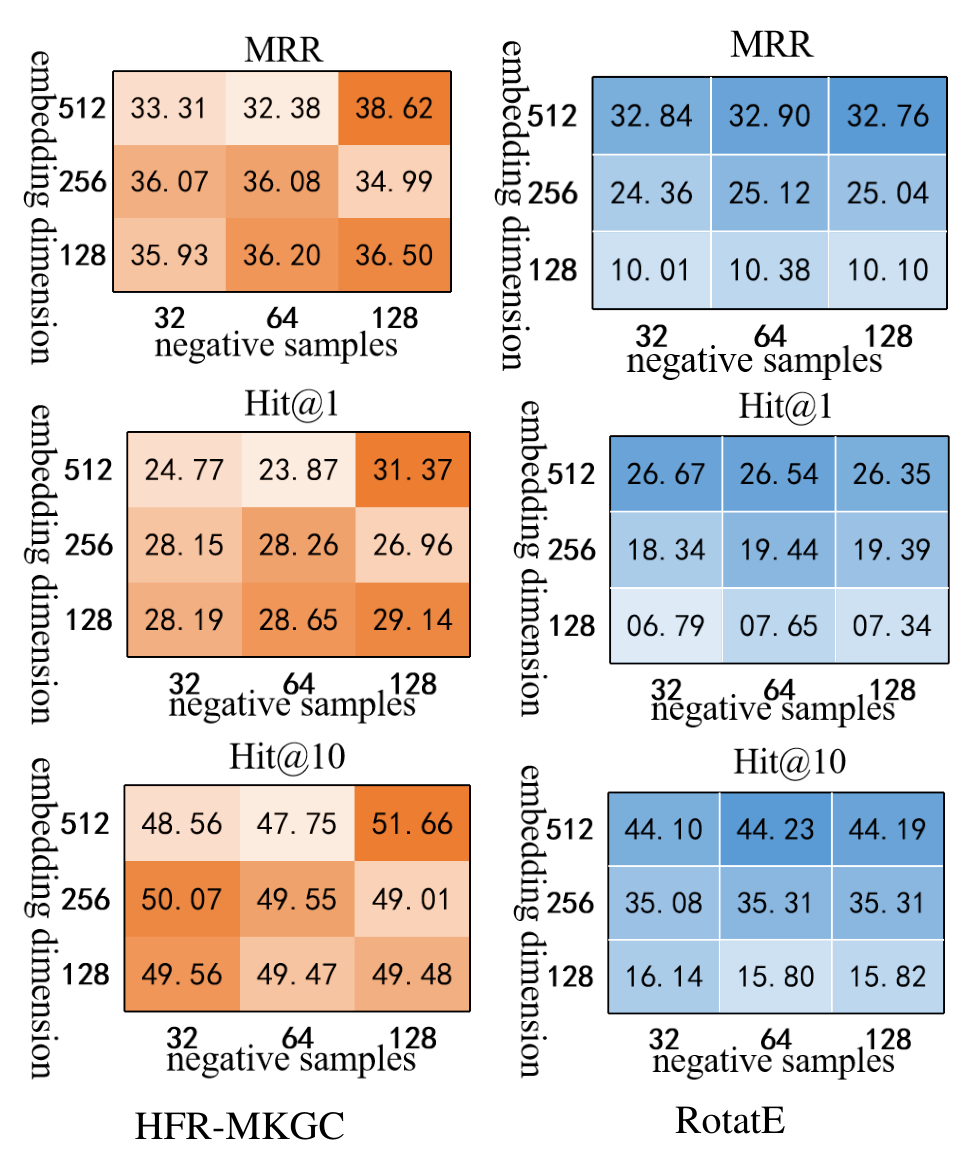
\includegraphics[width=0.95\linewidth]{fig3}
\caption{So sánh HFR-MKGC và RotatE trên MKG-W với các chiều embedding và số mẫu âm khác nhau. Màu đậm hơn nghĩa là hiệu năng tốt hơn.}
\label{fig:sensitivity}
\end{figure}

\subsection{Phân tích độ nhạy siêu tham số}

Chúng tôi phân tích ảnh hưởng của chiều embedding và số mẫu âm tới hiệu năng mô hình trên bộ MKG-W. Hình~\ref{fig:sensitivity} cho thấy kết quả với các tổ hợp khác nhau cho cả HFR-MKGC và RotatE. Ba quan sát chính nổi lên: (1) Chiều cao hơn (ví dụ 512) hưởng lợi nhiều hơn từ tập mẫu âm lớn (ví dụ 128), trong khi chiều trung bình (256) hoạt động tốt nhất với số mẫu âm vừa phải (64). Với chiều thấp (128), thay đổi số mẫu âm ảnh hưởng rất ít. (2) Chiều cao cần đủ mẫu âm. Không đủ mẫu âm, 256D có thể vượt 512D nhờ tối ưu tốt hơn. (3) Độ nhạy của các độ đo khác nhau. MRR và Hit@1 biến động nhiều hơn theo siêu tham số, trong khi Hit@10 tương đối ổn định. Các kết quả này gợi ý rằng việc tinh chỉnh cẩn thận cả hai siêu tham số là thiết yếu trong các mô hình đa phương thức.

\begin{figure}[t]
\centering
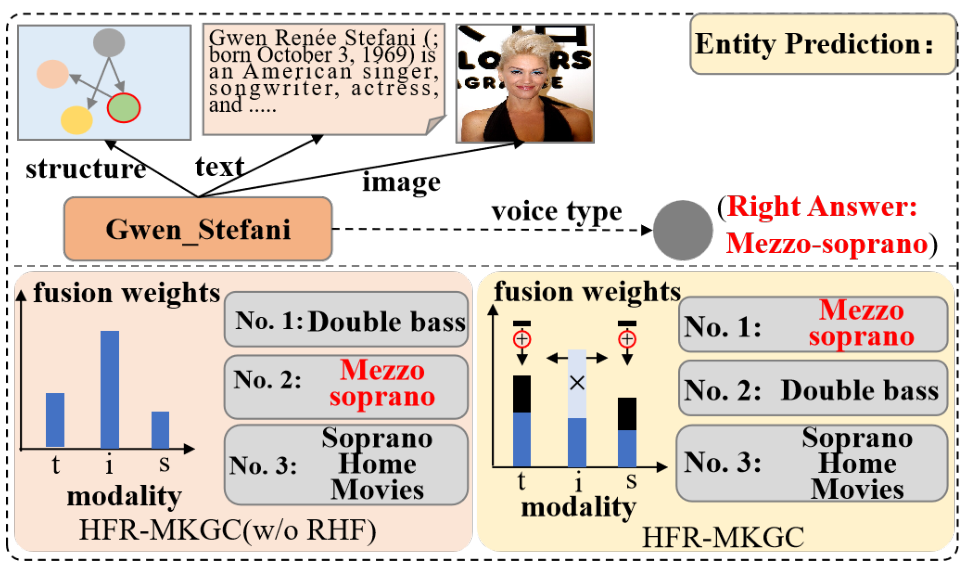
\includegraphics[width=\linewidth]{fig4}
\caption{Một ví dụ điển hình của HFR-MKGC. Biểu đồ cột biểu thị trọng số phương thức, các khối xám cho thấy thứ hạng ứng viên.}
\label{fig:case}
\end{figure}

\subsection{Nghiên cứu tình huống (Case Study)}

Để tìm hiểu thêm cách Hợp nhất phân cấp có dẫn hướng bởi quan hệ (RHF) tăng cường suy luận đa phương thức, chúng tôi thực hiện nghiên cứu tình huống định tính trên bộ MKG-W. Như Hình~\ref{fig:case}, chúng tôi chọn một bộ ba thiếu thực thể đuôi: (Gwen Stefani, voice type, ?). Chúng tôi so sánh kết quả suy diễn trong hai thiết lập: (1) HFR-MKGC w/o RHF, trong đó hợp nhất phương thức được thực hiện bằng trọng số khởi tạo ngẫu nhiên không có dẫn hướng bởi quan hệ; và (2) khung HFR-MKGC đầy đủ có RHF để gán trọng số thích ứng cho các phương thức dựa trên ngữ nghĩa quan hệ.

Kết quả cho thấy khi không có RHF, mô hình không ưu tiên được gợi ý phương thức đúng và chỉ xếp thực thể đích ``Mezzo-soprano'' ở vị trí thứ hai. Ngược lại, HFR-MKGC đặt nó đúng ở vị trí đầu. Lý do là ảnh của Gwen Stefani chỉ chứa thông tin ngoại hình, không có gợi ý thị giác nào về loại giọng, trong khi văn bản đi kèm gợi ý danh tính ca sĩ của cô. Vì vậy RHF gán trọng số cao hơn cho văn bản và thấp hơn cho ảnh qua Công thức~\ref{eq:2}--\ref{eq:3}, cho phép dự đoán chính xác ``Mezzo-soprano'' và xác nhận hiệu quả của thiết kế.

\section{Kết luận}

Trong bài báo này, chúng tôi đề xuất HFR-MKGC, một khung mới cho MMKGC. Phương pháp của chúng tôi đưa ra mô-đun hợp nhất phương thức phân cấp có dẫn hướng bởi quan hệ và tận dụng MLLM đã tinh chỉnh để suy diễn bộ ba theo chỉ dẫn. Hơn nữa, chúng tôi xây dựng các mẫu âm thách thức qua nhiễu loạn văn bản và nhiễu loạn thị giác, đồng thời tối ưu mô hình bằng huấn luyện đối kháng. Thực nghiệm rộng rãi trên nhiều bộ dữ liệu chuẩn xác nhận hiệu quả và ưu thế của phương pháp trong việc nắm bắt ngữ nghĩa đa phương thức và cải thiện hiệu năng suy luận. Trong tương lai, chúng tôi hướng tới khám phá cách sử dụng MLLM chính xác hơn cho biểu diễn và suy luận tri thức đa phương thức.

\section*{Lời cảm ơn}
Công trình này được hỗ trợ bởi National Key Research and Development Program of China (2023YFF0725103), National Natural Science Foundation of China (62192784, U22B2038, 62422202, 62272054), Beijing Nova Program (No. 20230484319).

\section*{Tài liệu tham khảo}
\small
\newcommand{\refitem}[1]{\par\noindent\hangindent=1.2em\hangafter=1 #1\par\vspace{1.5pt}}
\refitem{Barile, R.; d'Amato, C.; and Fanizzi, N. 2025. LP-DIXIT: Evaluating Explanations for Link Predictions on Knowledge Graphs using Large Language Models. In \textit{Proceedings of the ACM on Web Conference 2025}, 4034--4042.}
\refitem{Bordes, A.; Usunier, N.; Garcia-Duran, A.; Weston, J.; and Yakhnenko, O. 2013. Translating embeddings for modeling multi-relational data. \textit{Advances in Neural Information Processing Systems}, 26.}
\refitem{Chen, X.; Zhang, N.; Li, L.; Deng, S.; Tan, C.; Xu, C.; Huang, F.; Si, L.; and Chen, H. 2022. Hybrid transformer with multi-level fusion for multimodal knowledge graph completion. In \textit{Proceedings of the 45th International ACM SIGIR Conference on Research and Development in Information Retrieval}, 904--915.}
\refitem{Chen, Z.; Fang, Y.; Zhang, Y.; Guo, L.; Chen, J.; Pan, J. Z.; Chen, H.; and Zhang, W. 2025a. Noise-powered Multi-modal Knowledge Graph Representation Framework. In \textit{Proceedings of the 31st International Conference on Computational Linguistics}, 141--155.}
\refitem{Chen, Z.; Fang, Y.; Zhang, Y.; Guo, L.; Chen, J.; Pan, J. Z.; Chen, H.; and Zhang, W. 2025b. Noise-powered Multi-modal Knowledge Graph Representation Framework. In \textit{Proceedings of the 30th International Conference on Database Systems for Advanced Applications}.}
\refitem{Cui, Z.; Weng, Y.; Tang, X.; Lyu, F.; Liu, D.; He, X.; and Ma, C. 2025. Comprehending knowledge graphs with large language models for recommender systems. In \textit{Proceedings of the 48th International ACM SIGIR Conference on Research and Development in Information Retrieval}, 1229--1239.}
\refitem{Devlin, J.; Chang, M.-W.; Lee, K.; and Toutanova, K. 2019. BERT: Pre-training of deep bidirectional transformers for language understanding. In \textit{Proceedings of NAACL-HLT 2019, Volume 1 (Long and Short Papers)}, 4171--4186.}
\refitem{Fang, Y.; Fan, D.; Zha, D.; and Tan, Q. 2024. GAugLLM: Improving graph contrastive learning for text-attributed graphs with large language models. In \textit{Proceedings of the 30th ACM SIGKDD Conference on Knowledge Discovery and Data Mining}, 747--758.}
\refitem{Gao, Y.; Zhang, F.; Zhang, Z.; Min, X.; and Zhuang, F. 2025. Mixed-Curvature Multi-Modal Knowledge Graph Completion. In \textit{Proceedings of the AAAI Conference on Artificial Intelligence}, volume 39, 11699--11707.}
\refitem{Jian, Y.; Luo, X.; Li, Z.; Zhang, M.; Zhang, Y.; Xiao, K.; and Hou, X. 2025. APKGC: Noise-enhanced Multi-Modal Knowledge Graph Completion with Attention Penalty. In \textit{Proceedings of the AAAI Conference on Artificial Intelligence}, volume 39, 15005--15013.}
\refitem{Jiang, X.; Shen, Y.; Shi, Z.; Xu, C.; Li, W.; Li, Z.; Guo, J.; Shen, H.; and Wang, Y. 2024. Unlocking the Power of Large Language Models for Entity Alignment. In \textit{Proceedings of the 62nd Annual Meeting of the ACL (Volume 1: Long Papers)}, 7566--7583.}
\refitem{Kingma, D. P.; and Ba, J. 2015. Adam: A method for stochastic optimization. In \textit{Proceedings of the 3rd International Conference for Learning Representations}.}
\refitem{Li, A.; Li, Y.; Shao, Y.; and Liu, B. 2023. Multi-view scholar clustering with dynamic interest tracking. \textit{IEEE Transactions on Knowledge and Data Engineering}, 35(9): 9671--9684.}
\refitem{Li, M.; Yang, C.; Xu, C.; Song, Z.; Jiang, X.; Guo, J.; Leung, H.-f.; and King, I. 2025. Context-aware inductive knowledge graph completion with latent type constraints and subgraph reasoning. In \textit{Proceedings of the AAAI Conference on Artificial Intelligence}, volume 39, 12102--12111.}
\refitem{Li, Q.; Chen, Z.; Ji, C.; Jiang, S.; and Li, J. 2024. LLM-based multi-level knowledge generation for few-shot knowledge graph completion. In \textit{Proceedings of the 33rd International Joint Conference on Artificial Intelligence}, volume 3, 2135--2143.}
\refitem{Li, Y.; Yu, Z.; and He, D. 2024. Text-Rich Graph Neural Networks With Subjective-Objective Semantic Modeling. \textit{IEEE Transactions on Knowledge and Data Engineering}, 36(9): 4956--4967.}
\refitem{Liang, M.; Du, J.; Liang, Z.; Xing, Y.; Huang, W.; and Xue, Z. 2024a. Self-supervised multi-modal knowledge graph contrastive hashing for cross-modal search. In \textit{Proceedings of the AAAI Conference on Artificial Intelligence}, volume 38, 13744--13753.}
\refitem{Liang, M.; Li, Y.; Yu, Y.; Cao, X.; Xue, Z.; Li, A.; and Lu, K. 2024b. Structures aware fine-grained contrastive adversarial hashing for cross-media retrieval. \textit{IEEE Transactions on Knowledge and Data Engineering}, 36(7): 3514--3528.}
\refitem{Liu, H.; Li, C.; Wu, Q.; and Lee, Y. J. 2023. Visual instruction tuning. \textit{Advances in Neural Information Processing Systems}, 36: 34892--34916.}
\refitem{Liu, Q.; He, Y.; Xu, T.; Lian, D.; Liu, C.; Zheng, Z.; and Chen, E. 2024. UniMEL: A unified framework for multi-modal entity linking with large language models. In \textit{Proceedings of the 33rd ACM International Conference on Information and Knowledge Management}, 1909--1919.}
\refitem{Liu, Y.; Li, H.; Garcia-Duran, A.; Niepert, M.; Onoro-Rubio, D.; and Rosenblum, D. S. 2019. MMKG: multi-modal knowledge graphs. In \textit{European Semantic Web Conference}, 459--474. Springer.}
\refitem{Mousselly-Sergieh, H.; Botschen, T.; Gurevych, I.; and Roth, S. 2018. A multimodal translation-based approach for knowledge graph representation learning. In \textit{Proceedings of the Seventh Joint Conference on Lexical and Computational Semantics}, 225--234.}
\refitem{Pan, Y.; Hong, J.; Zhao, T.; Song, L.; Liu, J.; and Shang, X. 2025. Logic-Aware Knowledge Graph Reasoning for Structural Sparsity under Large Language Model Supervision. In \textit{Proceedings of the ACM on Web Conference 2025}, 4531--4542.}
\refitem{Panda, P.; Agarwal, A.; Devaguptapu, C.; Kaul, M.; and Ap, P. 2024. HOLMES: Hyper-Relational Knowledge Graphs for Multi-hop Question Answering using LLMs. In \textit{Proceedings of the 62nd Annual Meeting of the ACL (Volume 1: Long Papers)}, 13263--13282.}
\refitem{Radford, A.; Kim, J. W.; Hallacy, C.; Ramesh, A.; Goh, G.; Agarwal, S.; Sastry, G.; Askell, A.; Mishkin, P.; Clark, J.; et al. 2021. Learning transferable visual models from natural language supervision. In \textit{International Conference on Machine Learning}, 8748--8763. PMLR.}
\refitem{Sun, Z.; Deng, Z.-H.; Nie, J.-Y.; and Tang, J. 2019. RotatE: Knowledge Graph Embedding by Relational Rotation in Complex Space. In \textit{International Conference on Learning Representations}.}
\refitem{Touvron, H.; Martin, L.; Stone, K.; Albert, P.; Almahairi, A.; Babaei, Y.; Bashlykov, N.; Batra, S.; Bhargava, P.; Bhosale, S.; et al. 2023. Llama 2: Open foundation and fine-tuned chat models. \textit{arXiv preprint arXiv:2307.09288}.}
\refitem{Trouillon, T.; Welbl, J.; Riedel, S.; Gaussier, É.; and Bouchard, G. 2016. Complex embeddings for simple link prediction. In \textit{International Conference on Machine Learning}, 2071--2080. PMLR.}
\refitem{Wang, J.; Li, Y.; Shao, Y.; Xue, Z.; Guan, Z.; Li, A.; and Ye, G. 2025. Reinforcement Active Client Selection for Federated Heterogeneous Graph Learning. In \textit{Proceedings of the AAAI Conference on Artificial Intelligence}, volume 39, 21117--21125.}
\refitem{Wang, M.; Wang, S.; Yang, H.; Zhang, Z.; Chen, X.; and Qi, G. 2021. Is visual context really helpful for knowledge graph? A representation learning perspective. In \textit{Proceedings of the 29th ACM International Conference on Multimedia}, 2735--2743.}
\refitem{Wang, Z.; Li, L.; Li, Q.; and Zeng, D. 2019. Multimodal data enhanced representation learning for knowledge graphs. In \textit{2019 International Joint Conference on Neural Networks (IJCNN)}, 1--8. IEEE.}
\refitem{Xiao, S.; Shao, Y.; Li, Y.; Yin, H.; Shen, Y.; and Cui, B. 2022. LECF: recommendation via learnable edge collaborative filtering. \textit{Science China Information Sciences}, 65(1): 112101.}
\refitem{Xie, R.; Liu, Z.; Jia, J.; Luan, H.; and Sun, M. 2016. Representation learning of knowledge graphs with entity descriptions. In \textit{Proceedings of the AAAI Conference on Artificial Intelligence}, volume 30.}
\refitem{Xie, R.; Liu, Z.; Luan, H.; and Sun, M. 2017. Image-embodied Knowledge Representation Learning. In \textit{Proceedings of the Twenty-Sixth International Joint Conference on Artificial Intelligence}, 3140--3146.}
\refitem{Xu, D.; Xu, T.; Wu, S.; Zhou, J.; and Chen, E. 2022. Relation-enhanced negative sampling for multimodal knowledge graph completion. In \textit{Proceedings of the 30th ACM International Conference on Multimedia}, 3857--3866.}
\refitem{Yang, B.; Yih, S. W.-t.; He, X.; Gao, J.; and Deng, L. 2015. Embedding Entities and Relations for Learning and Inference in Knowledge Bases. In \textit{Proceedings of the International Conference on Learning Representations (ICLR) 2015}.}
\refitem{Yao, L.; Peng, J.; Mao, C.; and Luo, Y. 2025. Exploring large language models for knowledge graph completion. In \textit{ICASSP 2025 -- IEEE International Conference on Acoustics, Speech and Signal Processing}, 1--5. IEEE.}
\refitem{Zhang, R.; Su, Y.; Trisedya, B. D.; Zhao, X.; Yang, M.; Cheng, H.; and Qi, J. 2023. AutoAlign: Fully automatic and effective knowledge graph alignment enabled by large language models. \textit{IEEE Transactions on Knowledge and Data Engineering}, 36(6): 2357--2371.}
\refitem{Zhang, Y.; Chen, Z.; Guo, L.; Xu, Y.; Hu, B.; Liu, Z.; Zhang, W.; and Chen, H. 2024a. NativE: Multi-modal knowledge graph completion in the wild. In \textit{Proceedings of the 47th International ACM SIGIR Conference on Research and Development in Information Retrieval}, 91--101.}
\refitem{Zhang, Y.; Chen, Z.; Guo, L.; Xu, Y.; Hu, B.; Liu, Z.; Zhang, W.; and Chen, H. 2025. Tokenization, fusion, and augmentation: Towards fine-grained multi-modal entity representation. In \textit{Proceedings of the AAAI Conference on Artificial Intelligence}, volume 39, 13322--13330.}
\refitem{Zhang, Y.; Chen, Z.; Guo, L.; Xu, Y.; Zhang, W.; and Chen, H. 2024b. Making large language models perform better in knowledge graph completion. In \textit{Proceedings of the 32nd ACM International Conference on Multimedia}, 233--242.}
\refitem{Zhang, Y.; Chen, Z.; Liang, L.; Chen, H.; and Zhang, W. 2024c. Unleashing the Power of Imbalanced Modality Information for Multi-modal Knowledge Graph Completion. In \textit{Proceedings of LREC-COLING 2024}, 17120--17130.}
\refitem{Zhang, Y.; Chen, Z.; and Zhang, W. 2023. MACO: A modality adversarial and contrastive framework for modality-missing multi-modal knowledge graph completion. In \textit{CCF International Conference on Natural Language Processing and Chinese Computing}, 123--134. Springer.}
\refitem{Zhang, Z.; Wang, X.; Zhang, Z.; Li, H.; Qin, Y.; and Zhu, W. 2024d. LLM4DyG: can large language models solve spatial-temporal problems on dynamic graphs? In \textit{Proceedings of the 30th ACM SIGKDD Conference on Knowledge Discovery and Data Mining}, 4350--4361.}
\refitem{Zhao, Y.; Yu, J.; Cheng, Y.; Yu, C.; Liu, Y.; Li, X.; and Wang, S. 2025. Variational Graph Autoencoder for Heterogeneous Information Networks with Missing and Inaccurate Attributes. In \textit{Proceedings of the 31st ACM SIGKDD Conference on Knowledge Discovery and Data Mining V.1}, 2067--2078.}

\end{document}
